\documentclass[a4paper,12pt]{article}
\usepackage{xeCJK}
\usepackage{mylinuxfonts}
\usepackage{amsmath}
\usepackage{amsfonts}
\usepackage{amssymb}
\usepackage{mathrsfs}
\usepackage{amsbsy}
\usepackage{xcolor}
\usepackage{graphicx} % Allows including images
%\usepackage{multicol}

%%========================================

\begin{document}

\title{天线第一次作业}
\author{\textbf{刘洋} \\ 201428007326027 \\
liuyang614@mails.ucas.ac.cn\\{\kaishu{空间中心}}}
\date{2015-03-08}
\maketitle

% 以下为 作业内容
\newpage
\textcolor[rgb]{0,0,1}{\huge{第一题}}
\begin{flushleft} % 左对齐
用Matlab编程画出短振子的立体方向图和主平面极坐标的方向图。
\end{flushleft}


\begin{verse} 
theta=0:pi/50:pi;\\
phi=0:pi/50:2*pi;\\
r=sin(theta);\\
for i=1:length(phi)\\
%\hspace{1cm}x(i,:)=r.*sin(theta)*cos(phi(i));\\
$\quad$ x(i,:)=r.*sin(theta)*cos(phi(i));\\
$\quad$	y(i,:)=r.*sin(theta)*sin(phi(i));\\
$\quad$	z(i,:)=r.*cos(theta);\\
end\\
figure(1);\\
surf(x,y,z);\\
title('短振子立体方向图');\\
xlabel('x'),ylabel('y'),zlabel('z');\\
theta1=0:pi/50:2*pi;\\
r1=sin(theta1);\\
figure(2);\\
polar(theta1,abs(r1));\\

\end{verse}

%\begin{columns}
%\column{0.3\textwidth}




%\end{columns}








\begin{minipage}{0.5\textwidth}

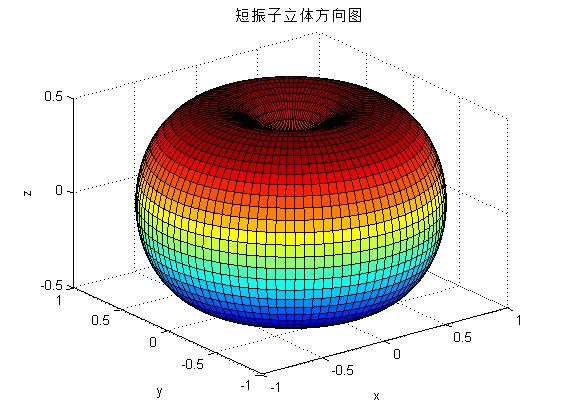
\includegraphics[width=\linewidth]{pictures/antenna_3dimension.jpg}
\end{minipage}%
\begin{minipage}{0.5\textwidth}
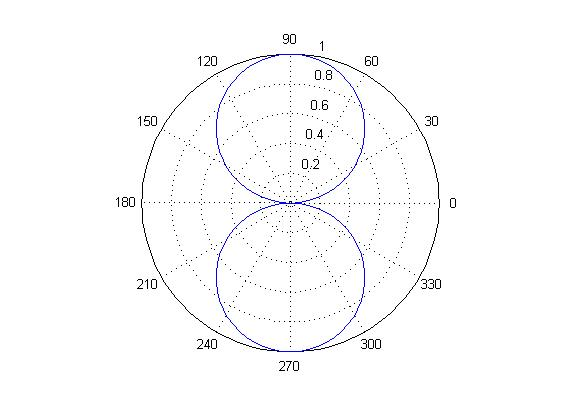
\includegraphics[width=\textwidth]{pictures/antenna_polar.jpg}%       
\end{minipage}





\newpage
\textcolor[rgb]{0,0,1}{\huge{第二题}}
\section{ 题~1.2.4}
\textbf{\kaishu{
电流元  最大方向$2\,km$ 电场强度 $E_0=1\,mV/m$。\\
1)最大方向$4\,km$处的电场强度$E_1$\\
2)~$E$面偏离最大方向$30^{\circ}$,$4\,km$处的磁场强度$H_2$。}}\\
\newline
解: 1)电流元在远场产生的电场的振幅为
$$E=\cfrac{60\pi IL}{\lambda r}sin\theta$$
\\
可见电场强度和距离成反比,当$r=2\,km$时,$E_0=1\,mV/m$,故当$r=4\,km$时,电场$E_1=0.5\,mV/m$。\\

~2)~$E$面偏离最大方向$30^{\circ}$且当$r=4\,km$时,电场强度的幅值为$$E_{\theta}=E_1 sin 30^{\circ}=0.5\times0.5=0.25\ mV/m$$
又有$$H_\phi=\cfrac{E_\theta}{120\pi}$$故磁场$$H_2=\cfrac{0.25\times 10^{-3}}{120\pi}=1.33\ \mu A/m$$


\section{题~1.2.5}
\textbf{\kaishu{电流元 $L=0.08\,\lambda$,电流为$5\,mA$时辐射功率。}}
\\
\newline
解:~电流元的辐射功率为%$$P_r=40\pi ^2(\cfrac{IL}{\lambda})^2=40\pi ^2(5\times 10^{-3}\cfrac{0.08\lambda}{\lambda})^2=$$
%%====================================================
%\begin{gather*}
%P_r=40\pi^2(\cfrac{IL}{\lambda})^2 \\
%=40\pi ^2(5\times 10^{-3}\cfrac{0.08\lambda}{\lambda})^2 \\
%\end{gather*}
%%==============================================
\begin{align*}
P_r &=40\pi^2(\cfrac{IL}{\lambda})^2 \\
&=40\pi ^2(5\times 10^{-3}\times\cfrac{0.08\lambda}{\lambda})^2 \\
&=6.317\times10^{-5}\ W \\
\end{align*}

\section{题~1.2.6}
\textbf{\kaishu{短振子长$L=1\,m$,$f=30\,MHz$,最大辐射方向$r=5\,km$处磁场振幅$H_0=5\times 10^{-4} \,A/m$,求电流振幅$I_0$和辐射功率。}}\\
\newline
解:~ 短振子远场区磁场振幅为$$H_0=\cfrac{I_0L}{4\lambda r}sin\theta$$由题意知,$L=1\,m$,$\lambda =\cfrac{v}{f}=\cfrac{3\times 10^8}{30\times 10 ^6}=10\,m$,$sin\theta =1$,$r=5\times 10^3\,m$故代入$H_0$得
\begin{align*}
I_0 &=\cfrac{4H_0\lambda r}{L sin\theta} \\
&=\cfrac{4\times 5\times 10^{-4}\times 10\times 5\times 10^3}{1\times 1} \\
&=100\ A \\
\end{align*}
辐射功率为
\begin{align*}
P_r &=10\pi ^2(\cfrac{I_0L}{\lambda})^2 \\
&=10\pi ^2(\cfrac{100\times 1}{10})^2 \\
&=9869.6\ W
\end{align*}

\section{题~1.2.7}
\textbf{\kaishu{全长为$L=\cfrac{\lambda}{2}$的半波对称振子的有效长度为$L_e=\cfrac{\lambda}{\pi}$,与全长为$L=0.1\,\lambda$的短振子相比,二者输入端电流$I_0$相同时,在远区相同距离处的最大场强比$E_M\text{(半)}/E_M\text{(短)}$。}}\\
\newline
解:~ 短振子的有效长度为其实际长度的一半,即$L_{es}=\cfrac{L}{2}=\cfrac{0.1\lambda}{2}=0.05\lambda$。又有$$E_M=\cfrac{60\pi I_0L_e}{\lambda r}$$
半波对称振子的有效长度和短振子的有效长度之比为$\cfrac{L_e}{L_{es}}=\cfrac{\lambda /2}{0.05\lambda}=10$,由电场表达式知,$$\cfrac{E_M\text{(半)}}{E_M\text{(短)}}=\cfrac{L_e}{L_{es}}=10$$
\section{题~1.2.8}
\textbf{\kaishu{短振子,全长$L=1.8\,m$,半径$a_0=2\,mm$,$\sigma=1.3\times 10^7\,S/m$。求$f=1\,MHz$时辐射效率$e_r$及输入电阻$R_{in}$。}}\\
\newline
解:~波长$\lambda=\cfrac{v}{f}=\cfrac{3\times 10^8}{10^6}=300\ m$, \\
辐射电阻为$R_{r0}=20\pi ^2(\cfrac{L}{\lambda})^2=20\pi ^2(\cfrac{1.8}{300})^2=0.0071\ \Omega$\\
$R_s=\sqrt{\cfrac{\pi \mu f}{\sigma}}=\sqrt{\cfrac{\pi \times 4\pi \times 10^{-7}\times 10^6}{1.3\times 10^7}}=5.511\times 10 ^{-4}\  \Omega$\\
损耗电阻为$R_{\sigma 0}=\cfrac{R_s}{2\pi a_0}\cfrac{L}{3}=\cfrac{5.511 \times 10^{-4}}{2\pi \times 2\times 10^{-3}}\times \cfrac{1.8}{3}=0.0263\ \Omega$\\
輻射效率为$e_r=\cfrac{P_r}{P_r+P_{\sigma}}=\cfrac{R_{r0}}{R_{r0}+R_{\sigma 0}}=\cfrac{0.0071}{0.0071+0.0263}=21.3\%$\\
\newline
输入电阻为$R_{in}=\cfrac{P_{in}}{I_0^2/2}=\cfrac{P_r+P_{\sigma}}{I_0^2/2}=R_{r0}+R_{\sigma 0}=0.0334\ \Omega$
\end{document}